\documentclass[189]{pset}

% ================================================================== %
%                                                                    %
%                              Document                              %
%                                                                    %
% ================================================================== %

% ----------------------- Header formatting ------------------------ %

\name{Forest Kobayashi}
\class{Math of Big Data}
\season{Summer}
\prof{Gu}
\assignment{6}
\duedate{05/22/2018}
\dueday{Tuesday}
\problems{1, 2}
\acknowledgements{{}, {}}
\onTime{0}

\comments{\textbf{Comments:} Feel free to work with other students,
  but make sure you write up the homework and code on your own (no
  copying homework \textit{or} code; no pair programming). Feel free
  to ask students or instructors for help debugging code or whatever
  else, though.

  The starter files for problem 2 can be found under the Resource tab
  on course website. Please print out all the graphs generated by your
  own code and submit them together with the written part, and make
  sure you upload the code to your Github repository. }

\lfoot{Due Tuesday, May 22nd 2018}

\begin{document}

% --------------------------- Problem 1 ---------------------------- %

  \section{(Murphy 11.2)}
    \textbf{(EM for Mixtures of Gaussians)} Show that the M step for
    ML estimation of a mixture of Gaussians is given by
    \begin{align*}
      \bm{\mu}_k
      &= \frac{\sum_i r_{ik}\vx_i}{r_k} \\
      \bm{\Sigma}_k
      &= \frac{1}{r_k}\sum_i r_{ik}(\vx_i - \bm{\mu}_k)(\vx_i -
        \bm{\mu}_k)^\T \\
      &= \frac{1}{r_k} \sum_i r_{ik}\vx_i\vx_i^\T - r_k\bm{\mu}_k
        \bm{\mu}_k^\T.
    \end{align*}

  \hrulefill

  \section*{Solution:}
    % Our EM algorithm can be described as follows:
    % \begin{enumerate}[label=\arabic*.]
    %   \item Repeat the following until convergence:
    %   \item (E-step) $\forall i$, $Q_i \pn{z^{(i)}} \coloneqq
    %     p(z^{(i)} \mid x^{(i)}; \theta)$
    %   \item (M-step) set
    %     \[
    %       \theta \coloneqq \argmax_{\theta} \sum_i \sum_{z^(i)}
    %       Q_i(z^{(i)}) \log \pn{\frac{p(x^{(i)}, z^{(i)}; \theta)}{Q_i
    %           (z^{(i)})}}
    %     \]
    %     where $Q_i(z)$ is
    %   \end{enumerate}

    In the M-step, we want to optimize
    \begin{align*}
      \ell(\bm{\mu}_k, \bm{\Sigma}_k )
      &= \sum_k \sum_i r_{ik} \log p(\vx_i \mid \bm{\theta}_k) \\
      &= -\frac{1}{2} \sum_i r_{ik} \bk{\log \abs{\Sigma_k} + (\vx_i -
        \bm{\mu}_k)^\T \bm{\Sigma}_k^{-1} (\vx_i - \bm{\mu}_k)}
    \end{align*}
    we first calculate the optimal $\bm{\mu}_k$:
    \begin{align*}
      \pd{\ell(\bm{\mu}_k, \bm{\Sigma}_k)}{\bm{\mu}_k}
      &= -\frac{1}{2} \sum_i -2r_{ik} \bm{\Sigma}_k^{-1} (\vx_i -
        \bm{\mu}_k) \\
      &= \sum_i r_{ik} \bm{\Sigma}_k^{-1} (\vx_i - \bm{\mu}_k) \\
      &= 0
    \end{align*}
    thus
    \begin{align*}
      \sum_i r_{ik} \bm{\Sigma}_k^{-1} \vx_i
      &= \sum_i r_{ik} \bm{\Sigma}_k^{-1} \bm{\mu}_k \\
      \sum_i r_{ik} \vx_i
      &= \sum_i r_{ik} \bm{\mu}_k \\
      \boxed{\frac{\sum_i r_{ik} \vx_i}{\sum_i r_{ik}}}
      &= \bm{\mu}_k
    \end{align*}
    as desired. Note that
    \[
      \pd{\va^\T \bX^{-1}\vb}{\bX} = -\bX^{-\T} \va \vb^\T \bX^{-\T}
    \]
    Hence, differentiating with respect to $\bm{\Sigma}_k$, we have
    \begin{align*}
      \pd{\ell(\bm{\mu_k}, \bm{\Sigma}_k)}{\bm{\Sigma}_k}
      &= -\frac{1}{2} \sum_i r_{ik} \bk{\bm{\Sigma}_k^{-\T}
        -\bm{\Sigma}_k^{-\T} \pn{\vx_i - \bm{\mu}_k} \pn{\vx_i -
        \bm{\mu}_k}^{\T} \bm{\Sigma}_k^{-\T}} \\
      &= -\frac{1}{2} \sum_i r_{ik} \bk{\bm{\Sigma}_k^{-1} -
        \Sigma^{-1}_k (\vx_i - \bm{\mu}_k)(\vx_i - \bm{\mu}_k)^{\T}
        \bm{\Sigma}_k^{-1}}
    \end{align*}
    and so
    \begin{align*}
      \sum_i r_{ik} \bm{\Sigma}_k^{-1}
      &= \sum_i r_{ik} \bm{\Sigma}_k^{-1} (\vx_i - \bm{\mu}_k)(\vx_i -
        \bm{\mu}_k)^{\T} \bm{\Sigma}_k^{-1} \\
      \sum_i r_{ik}
      &= \sum_i r_{ik} \bm{\Sigma}_k^{-1} (\vx_i - \bm{\mu}_k)(\vx_i -
        \bm{\mu}_k)^{\T} \\
      \bm{\Sigma}_k
      &= \frac{\sum_i r_{ik} (\vx_i - \bm{\mu}_k)(\vx_i -
        \bm{\mu}_k)^{\T}}{\sum_i r_{ik}}
    \end{align*}
  \clearpage

% --------------------------- Problem 2 ---------------------------- %

  \section{(SVD Image Compression)}
    In this problem, we will use the image of a scary clown online to
    perform image compression.  In the starter code, we have already
    load the image into a matrix/array for you. However, you might
    need internet connection to access the image and therefore
    successfully run the starter code. The code requires Python
    library Pillow in order to run.

    Plot the progression of the 100 largest singular values for the
    original image and a randomly shuffled version of the same image
    (all on the same plot). In a single figure plot a grid of four
    images: the original image, and a rank $k$ truncated SVD
    approximation of the original image for $k \in \set{2,10,20}$.

  \hrulefill

  \section*{Solution:}
  \begin{figure}[H]
    \centering
    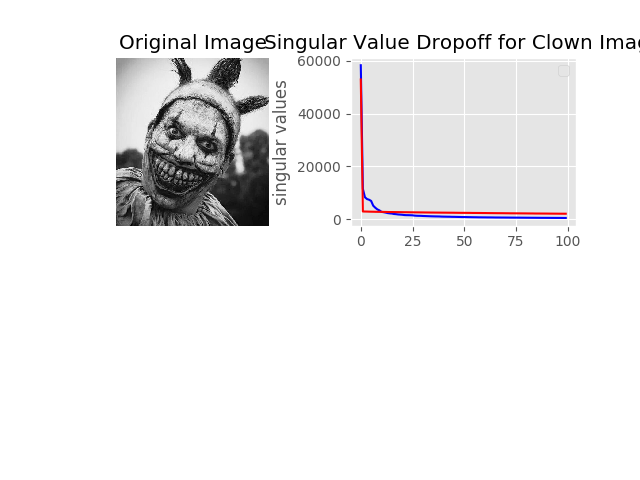
\includegraphics{dropoff.png}
    \caption{Dropoff}
    \label{fig:drop}
  \end{figure}
  \begin{figure}[H]
    \centering
    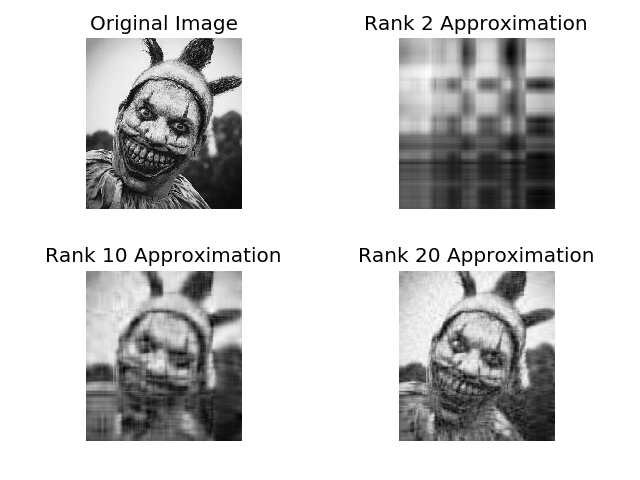
\includegraphics{reconstruction.png}
    \caption{Reconstruction}
    \label{fig:rec}
  \end{figure}
\end{document}
